% Compilation : pdflatex Mecanique_terrestre.tex (deux fois).
% Document autonome : texte, formules et figures TikZ modifiables.
% Les reperes Source renvoient aux pages du manuscrit.
\documentclass[11pt,a4paper]{article}
\usepackage[utf8]{inputenc}
\usepackage[T1]{fontenc}
\usepackage[provide=*,french]{babel}
\usepackage[scaled=.95]{helvet}
\renewcommand{\familydefault}{\sfdefault}
\usepackage{amsmath,amssymb,esint,array,tabularx}
\usepackage{geometry}
\geometry{left=15mm,right=15mm,top=18mm,bottom=18mm,headheight=14pt,headsep=6mm}
\usepackage{fancyhdr,lastpage,tikz}
\usetikzlibrary{arrows.meta,calc,decorations.pathreplacing,decorations.pathmorphing,decorations.markings,patterns}
\usepackage[most]{tcolorbox}
\usepackage{enumitem,titlesec,needspace,hyperref}
\hypersetup{hidelinks,pdftitle={Mécanique terrestre},pdfsubject={Cours de physique}}
\pagestyle{fancy}\fancyhf{}
\fancyhead[L]{\small Physique M4 - Mécanique terrestre - inspiré par les cours de Mme Mesnil}
\fancyhead[R]{\small\thepage/\pageref{LastPage}}
\fancyfoot[R]{\small PC-PC*}
\renewcommand{\headrulewidth}{0pt}
\clubpenalty=10000\widowpenalty=10000\displaywidowpenalty=10000
\setlength{\parindent}{0pt}\setlength{\parskip}{5pt}
\setlength{\abovedisplayskip}{7pt}\setlength{\belowdisplayskip}{7pt}
\setlist[itemize]{leftmargin=5mm,itemsep=3pt,topsep=3pt,label=\(\rightarrow\)}
\setlist[enumerate]{leftmargin=6mm,itemsep=3pt,topsep=3pt}
\renewcommand{\thesection}{\Roman{section}}
\renewcommand{\thesubsection}{\thesection.\arabic{subsection}}
\titleformat{\section}{\Large\bfseries}{\thesection.}{.4em}{}
\titleformat{\subsection}{\large\bfseries}{\thesubsection.}{.4em}{}[\titlerule]
\titleformat{\subsubsection}{\normalsize\bfseries}{\alph{subsubsection})}{.5em}{}
\titlespacing*{\section}{0pt}{11pt}{6pt}
\titlespacing*{\subsection}{0pt}{9pt}{5pt}
\titlespacing*{\subsubsection}{0pt}{8pt}{4pt}
\newtcolorbox{cadre}[1][]{enhanced,sharp corners,colback=white,colframe=black,boxrule=1.1pt,left=7pt,right=7pt,top=5pt,bottom=5pt,before skip=7pt,after skip=7pt,#1}
\newtcolorbox{exemple}[1][]{enhanced,sharp corners,colback=white,colframe=black,boxrule=.7pt,left=8pt,right=8pt,top=6pt,bottom=6pt,before skip=8pt,after skip=8pt,#1}
\tcbset{etoiles/.style={width=\dimexpr\linewidth-22mm\relax,overlay={\node[anchor=west,inner sep=0pt,font=\small] at ([xshift=2mm]frame.east) {\(#1\)};}}}
\newcommand{\dd}{\mathrm d}
\newcommand{\vv}{\vec v}
\newcommand{\grad}{\overrightarrow{\mathrm{grad}}}
\newcommand{\pd}[2]{\frac{\partial #1}{\partial #2}}
\newcommand{\ux}{\vec u_x}\newcommand{\uy}{\vec u_y}\newcommand{\uz}{\vec u_z}
\newcommand{\cste}{\mathrm{cste}}
\newcommand{\titr}[1]{\par\textbf{\underline{#1}}\par\nopagebreak[3]}
\newcommand{\planpart}[2]{\par\vspace{5pt}{\bfseries #1. #2}\par}
\newcommand{\plansub}[2]{\hspace*{7mm}{\itshape #1) #2}\par}
\newcommand{\plansubsub}[1]{\hspace*{15mm}{\itshape #1}\par}
\tikzset{>=Stealth,every node/.style={font=\small},flow/.style={thick,->},edge/.style={thick}}
\newcommand{\etoiles}[1]{\foreach \i in {1,...,#1}{\mathord{\star}\,}}
\newcommand{\R}{\mathcal R}
\newcommand{\RT}{\R_T}\newcommand{\RH}{\R_H}\newcommand{\RG}{\R_{\text{géo}}}
\newcommand{\Om}{\vec\Omega_{\RT/\RG}}\newcommand{\om}{\Omega_{\RT/\RG}}
\newcommand{\Fie}{\vec F_{\mathrm{ie}}}\newcommand{\Fic}{\vec F_{\mathrm{ic}}}\newcommand{\Fd}{\vec F_{\mathrm{div}}}
\newcommand{\HM}{\overrightarrow{HM}}\newcommand{\ur}{\vec u_r}
\newcommand{\rep}[1]{\draw[->] (0,0)--(1,0);\draw[->] (0,0)--(0,1);\draw[->] (0,0)--(-.5,-.55);\node[below right] at (.3,-.15){$#1$};}
\newcommand{\pointgrav}{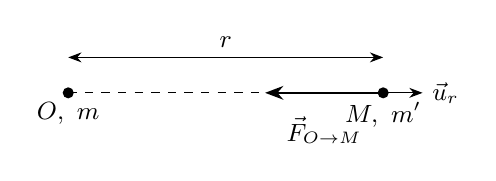
\begin{tikzpicture}
\fill (0,0) circle(2pt) node[below]{$O,\ m$};\fill (4,0) circle(2pt) node[below]{$M,\ m'$};
\draw[dashed] (0,0)--(4,0);\draw[<->] (0,.45)--(4,.45) node[midway,above]{$r$};
\draw[->,thick] (4,0)--(2.5,0) node[midway,below=5pt]{$\vec F_{O\to M}$};\draw[->] (4,0)--(4.5,0) node[right]{$\ur$};\end{tikzpicture}}
% Terre, axe polaire, latitude et forces (1 : force centrifuge ; 2 : pesanteur).
\newcommand{\terre}[1]{\begin{tikzpicture}[scale=.95]
\draw[thick] (0,0) circle(1.35);\fill (0,0) circle(1.5pt) node[below left]{$T$};
\draw[dashed] (-1.65,0)--(1.7,0);\draw[->] (0,-1.6)--(0,2) node[above]{$\Delta$};
\ifnum#1=1\coordinate (M) at (40:1.35);\else\coordinate (M) at (40:1.65);\fi
\draw[dashed] (0,0)--(M);\fill (M) circle(1.7pt) node[above right,xshift=1pt,yshift=1pt]{$M$};
\draw (.43,0) arc(0:40:.43);
\ifnum#1=2
\node at (.7,-.55){$\lambda$};\draw[thin] (.67,-.38)--(.38,.12);
\else\node at (.72,.16){$\lambda$};\fi
\ifnum#1=1
\draw[dashed] (0,.868)--(M);\node[left] at (0,.868){$H$};\draw (0,.7)--(.16,.7)--(.16,.868);
\fi
\draw[->,thick] (M)--($(M)!.52!(0,0)$);\node[above left,inner sep=3pt] at (.95,.79){$\vec g_T$};
\draw[->,thick] (M)--++(.85,0) node[right]{$\ifnum#1=1\Fie\else\Omega^2\HM\fi$};
\ifnum#1=2
\draw[->,thick] (M)--++(-.3,-.72) node[right]{$\vec g$};
\draw[->,thick] (0,1.35)--(0,.65) node[left]{$\vec g$};
\draw[->,thick] (1.35,0)--(.65,0) node[below,midway]{$\vec g$};
\fi
\end{tikzpicture}}
\newcommand{\orbite}[1]{\begin{tikzpicture}[scale=.8]
\draw[dashed] (0,0) ellipse(3 and 1.7);
\fill (0,0) circle(2pt);\node[above left,xshift=-3pt,yshift=2pt] at (0,0){$S$};\rep{\RH}
\coordinate (T) at (2.6,.85);\draw[dotted] (0,0)--(T);\fill (T) circle(2pt) node[below left,xshift=-2pt,yshift=-2pt]{$T$};
\begin{scope}[shift={(T)}]\rep{\RG}\draw (0,0) circle(.32);\end{scope}
\begin{scope}[shift={(T)},rotate=35]
\draw[->,thick] (0,0)--(1.75,0);
\draw[->,thick] (0,0)--(0,1.75) node[above]{$\Delta$};
\draw[->,thick] (0,0)--(-.95,-1.045);
\end{scope}
\node[right] at (4.15,1.95){$\RT$};\draw[->] (-2.7,-.9) arc(210:240:3 and 1.7);
\ifnum#1=1
\begin{scope}[rotate=18.103]\draw[->] (0,0)--(1.7,0);\draw[->] (0,0)--(0,1.7);\end{scope}
\node[above] at (1.65,.63){$\R'$};
\fi
\end{tikzpicture}}
\newcommand{\pendule}{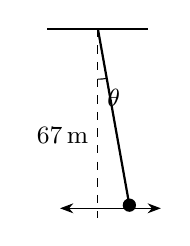
\begin{tikzpicture}[scale=.8]
\draw[thick] (-.8,0)--(.8,0);\draw[dashed] (0,0)--(0,-3);\draw[thick] (0,0)--(.5,-2.8);\fill (.5,-2.8) circle(3pt);
\draw (0,-.8) arc(270:280:.8);\node at (.25,-1.1){$\theta$};\node[left] at (0,-1.7){$67\,\mathrm m$};\draw[<->] (-.6,-2.85)--(1,-2.85);\end{tikzpicture}}
% Champ gravitationnel (0) puis champ differentiel (1,2) ; 2 ajoute les bourrelets.
\newcommand{\maree}[1]{\begin{tikzpicture}[scale=.9]
\draw[thick] (0,0) circle(1.25);\fill (0,0) circle(1.5pt) node[below left]{$T$};\draw[dotted] (-1.3,0)--(5,0);\draw (5,0) circle(.22);\node[right] at (5.25,0){$\ifnum#1=2 L\else A\fi$};
\ifnum#1<2\draw[->] (0,0)--(55:1.25) node[midway,left]{$R_T$};\fi
\ifnum#1=0
\foreach \a/\l in {180/.45,0/1,55/.7,-55/.7}{\draw[->,thick] (\a:1.25)--($(\a:1.25)!\l cm!(5,0)$);}\draw[->,thick] (0,0)--(.7,0);
\else
\foreach \a in {0,45,90,135,180,225,270,315}{\draw[->,thick] (\a:1.25)--++({.55*cos(\a)},{-.3*sin(\a)});}
\ifnum#1=1\node[below left] at (-1.25,0){$P$};\node[below right] at (1.25,0){$Q$};\fi
\fi
\draw[dotted] (55:1.25)--(5,0)--(-55:1.25);
\ifnum#1=2\draw[thick] (0,0) ellipse(1.85 and 1.3);\node[below,align=center] at (0,-1.6){Deux bourrelets océaniques};\fi
\end{tikzpicture}}
\begin{document}
{\raggedright\fontsize{27}{31}\selectfont\bfseries Mécanique terrestre\par}
\vspace{4mm}
\begingroup\setlength{\parskip}{.7pt}
\planpart{I}{Le champ de gravitation}
\plansub{1}{Force et champ de gravitation créés par un point matériel}
\plansub{2}{Énergie potentielle et potentiel gravitationnel}
\plansub{3}{Champ de gravitation à la surface de la Terre}
\planpart{II}{La dynamique terrestre}
\plansub{1}{Choix des référentiels}
\plansub{2}{La relation fondamentale de la dynamique}
\planpart{III}{Champ de pesanteur terrestre}
\plansub{1}{Définition}
\plansub{2}{Conséquences}
\planpart{IV}{Influence de la force de Coriolis}
\plansub{1}{Quelques généralités}
\plansub{2}{Déviation vers l'est}
\plansub{3}{Pendule de Foucault}
\plansub{4}{Anticyclones-dépressions}
\planpart{V}{Effets de marées}
\plansub{1}{Le terme des marées}
\plansub{2}{Théorie statique des marées}
\endgroup

% Source 1
\section{Le Champ de gravitation}
\subsection{Force et champ de gravitation créés par un point matériel}
\begin{center}\pointgrav\end{center}
\begin{cadre}\[\vec F_{O\to M}=-\frac{Gmm'}{r^2}\ur\]\textbf{Loi de Newton.}\end{cadre}
La force s'écrit $\vec F_{O\to M}=m'\vec g(M)$, où $\vec g(M)$ est le champ de gravitation créé en $M$ par le point matériel de masse $m$ situé en $O$.
\begin{cadre}\[\vec g(M)=-\frac{Gm}{r^2}\ur=-\frac{Gm}{OM^3}\overrightarrow{OM}.\]\end{cadre}
Il s'agit d'un champ vectoriel.

% Source 2
\subsection{Énergie potentielle et potentiel gravitationnel}
\begin{center}\pointgrav\end{center}
Dans le référentiel lié à $O$, en coordonnées sphériques,
\[\vec F_{O\to M}=-\frac{Gmm'}{r^2}\ur=-\grad E_p.\]
\begin{cadre}\[E_p=-\frac{Gmm'}r+\cste\]\textbf{Énergie potentielle de gravitation.}\end{cadre}
Les composantes du gradient sont
\[\grad E_p=\begin{pmatrix}\displaystyle\pd{E_p}{r}\\[12pt]\displaystyle\frac1r\pd{E_p}{\theta}=0\\[12pt]\displaystyle\frac1{r\sin\theta}\pd{E_p}{\varphi}=0\end{pmatrix}_{(\ur,\vec u_\theta,\vec u_\varphi)}.\]
\begin{cadre}\[V(M)=-\frac{Gm}r+\cste\]\end{cadre}
$V(M)$ est le potentiel gravitationnel créé en $M$ par la masse $m$ située en $O$.
\[E_p(M)=m'V(M).\]

% Sources 3-4
\subsection{Champ de gravitation à la surface de la Terre}
Le champ de gravitation terrestre peut-il être considéré comme quasi uniforme ?
\begin{center}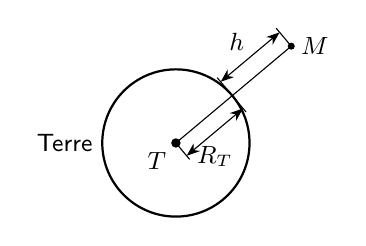
\begin{tikzpicture}[scale=.85]
\draw[thick] (0,0) circle(1.1);\fill (0,0) circle(2pt) node[below left]{$T$};
\coordinate (A) at (40:1.1);\coordinate (M) at (40:2.25);\draw (0,0)--(M);\fill (M) circle(1.5pt) node[right]{$M$};
\begin{scope}[rotate=40]
\draw[thin] (0,0)--(0,-.32);\draw[thin] (1.1,0)--(1.1,-.32);
\draw[<->] (0,-.25)--(1.1,-.25) node[midway,below=3pt,inner sep=2pt]{$R_T$};
\draw[thin] (1.1,0)--(1.1,.35);\draw[thin] (2.25,0)--(2.25,.35);
\draw[<->] (1.1,.27)--(2.25,.27) node[midway,above left,inner sep=2pt]{$h$};
\end{scope}\node[left] at (-1.1,0){Terre};
\end{tikzpicture}\end{center}
\textbf{Hypothèse :} la Terre présente une répartition de masse à symétrie sphérique : la masse volumique vérifie $\mu=\mu(r)$.
Le champ extérieur est le même que si toute la masse $M_T$ était concentrée au centre $T$.
\begin{center}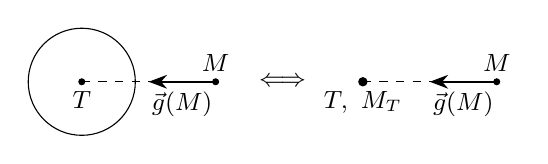
\begin{tikzpicture}[scale=.85]
\draw (0,0) circle(.8);\fill (0,0) circle(1.5pt) node[below]{$T$};\draw[dashed] (0,0)--(2,0);\fill (2,0) circle(1.5pt) node[above]{$M$};\draw[->,thick] (2,0)--(1,0) node[midway,below]{$\vec g(M)$};\node at (3,0){$\Longleftrightarrow$};
\fill (4.2,0) circle(2pt) node[below]{$T,\ M_T$};\draw[dashed] (4.2,0)--(6.2,0);\fill (6.2,0) circle(1.5pt) node[above]{$M$};\draw[->,thick] (6.2,0)--(5.2,0) node[midway,below]{$\vec g(M)$};
\end{tikzpicture}\end{center}
\begin{cadre}\[\vec g(M)=-\frac{GM_T}{r^2}\ur.\]\end{cadre}
Cf. théorème de Gauss en électromagnétisme.
\[\vec g(M)=-\frac{GM_T}{(R_T+h)^2}\ur,\qquad R_T=6700\,\mathrm{km},\quad h\ll R_T.\]
\begin{align*}
\|\vec g(M)\|&=\frac{GM_T}{R_T^2}\left(1+\frac h{R_T}\right)^{-2}\\
&\simeq\frac{GM_T}{R_T^2}\left(1-\frac{2h}{R_T}\right)
=\|\vec g(h=0)\|\left(1-\frac{2h}{R_T}\right).
\end{align*}
\[\left|\frac{\|\vec g(h)\|-\|\vec g(h=0)\|}{\|\vec g(h=0)\|}\right|\simeq\frac{2h}{R_T}.\]
Pour $\Delta g/g=1\,\%$, on obtient $h\simeq30\,\mathrm{km}$. Dans les expériences usuelles, la norme du champ de gravitation est uniforme.

% Sources 5-9
\section{La dynamique terrestre}
\subsection{Choix des référentiels}
\begin{itemize}
\item Le référentiel d'étude $\RT$, terrestre, est lié à la Terre. Son origine est $T$ ou un point de la surface terrestre ; ses trois axes sont liés à la Terre.
\item Le référentiel héliocentrique $\RH$ a pour origine le centre $S$ du Soleil. Ses axes sont dirigés vers trois points fixes.
\item Le référentiel géocentrique $\RG$ a pour origine le centre $T$ de la Terre. Ses axes sont dirigés vers les mêmes trois points fixes.
\end{itemize}
\begin{center}\orbite{0}\end{center}
$\RG$ est en translation circulaire par rapport à $\RH$ : $\vec\Omega_{\RG/\RH}=\vec0$. En supposant $\RH$ galiléen, on peut étudier la dynamique dans $\RG$.

$\RT$ est en rotation autour de l'axe $\Delta$ dans $\RG$. Le vecteur $\Om$ est non nul et parallèle à $\Delta$.
En supposant $\RG$ galiléen, on étudie la dynamique dans $\RT$, en rotation uniforme autour de $\Delta$, fixe dans $\RG$. On suppose $\Om$ constant.

Cette hypothèse néglige la précession de $\Delta$, de période d'environ $26\,000$ ans, et ses oscillations de $20''$, de période d'environ $18$ ans.

\titr{Détermination de $\Om$}
Le jour solaire, de durée $T_{\mathrm{sol}}=24\,\mathrm h$, est la durée entre deux passages successifs du Soleil au méridien d'un même point terrestre.
\begin{center}\orbite{1}\end{center}
On introduit $\R'$, d'origine $S$, dont un axe reste porté par $ST$ ; les deux autres axes complètent une base orthonormée. Ce référentiel tourne autour de $Sz$ :
\[\vec\Omega_{\R'/\RH}=\frac{2\pi}{T_{\mathrm{an}}}\uz.\]
Dans $\R'$, le référentiel terrestre tourne autour de $\Delta$, fixe :
\[\vec\Omega_{\RT/\R'}=\frac{2\pi}{T_{\mathrm{sol}}}\vec u_\Delta.\]
La composition des vecteurs rotation donne
\[\vec\Omega_{\RT/\RH}=\Om+\underbrace{\vec\Omega_{\RG/\RH}}_{\vec0\text{ : translation}},\]
\[\text{puis}\qquad\Om=\vec\Omega_{\RT/\RH}=\vec\Omega_{\RT/\R'}+\vec\Omega_{\R'/\RH}.\]
On suppose $\Delta$ parallèle à $\uz$, en négligeant l'inclinaison de $23^\circ$. Ainsi,
\[\Om=\left(\frac{2\pi}{T_{\mathrm{sol}}}+\frac{2\pi}{T_{\mathrm{an}}}\right)\uz=\frac{2\pi}{T_{\mathrm{sid}}}\uz.\]
\begin{cadre}\[\frac1{T_{\mathrm{sid}}}=\frac1{T_{\mathrm{sol}}}+\frac1{T_{\mathrm{an}}}.\]\end{cadre}
Avec $T_{\mathrm{sol}}=24\,\mathrm h$ et $T_{\mathrm{an}}=365{,}25\,\text{jours}$,
\begin{cadre}[etoiles={\etoiles{1}}]\[T_{\mathrm{sid}}=23\,\mathrm h\,56'\qquad\text{(jour sidéral)}.\]\end{cadre}
\[\Omega=7{,}3\times10^{-5}\,\mathrm{rad\,s^{-1}}.\]
En conclusion, $\Om=\vec\Omega_{\RT/\RH}=\dfrac{2\pi}{T_{\mathrm{sid}}}\uz$.

\subsection{La relation fondamentale de la dynamique}
On suppose $\RG$ galiléen. Le référentiel $\RT$ est non galiléen, en rotation uniforme autour de l'axe des pôles $\Delta$. Le système étudié est un point matériel $M$ de masse $m$.
\[m\vec a_{\RT}(M)=m\vec g_T(M)+\Fd+\Fie+\Fic,\]
où $\Fd$ représente les autres forces.
\begin{cadre}\[m\vec a_{\RT}(M)=m\vec g_T(M)+\Fd+m\om^2\HM-2m\Om\wedge\vec v_{\RT}(M).\]\end{cadre}
$H$ est le projeté orthogonal de $M$ sur $\Delta$.
\begin{center}\terre{1}\quad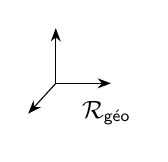
\begin{tikzpicture}[scale=.7]\rep{\RG}\end{tikzpicture}\end{center}
\textbf{Remarque.} On néglige les effets gravitationnels du Soleil et des autres planètes, ce qui est lié à l'hypothèse d'un référentiel géocentrique galiléen.
% Sources 10-15
\section{Champ de pesanteur terrestre}
\subsection{Définition}
Pour maintenir un point matériel en équilibre à la surface de la Terre, on doit appliquer une force $\vec F$ : réaction d'un support, tension d'un fil ou effort musculaire, par exemple. Le poids est l'opposé de cette force.

Considérons un point matériel $M$, de masse $m$, à l'équilibre dans $\RT$ :
\[\vec0=m\vec g_T(M)+\vec F+m\om^2\HM+\vec0.\]
\begin{cadre}[etoiles={\etoiles{3}}]\[\vec P=-\vec F=m\vec g_T(M)+m\om^2\HM.\]\end{cadre}
Le champ de pesanteur terrestre $\vec g$ est défini par $\vec P=m\vec g$.
\begin{cadre}[etoiles={\etoiles{4}}]\[\vec g(M)=\vec g_T(M)+\om^2\HM.\]\end{cadre}
\begin{center}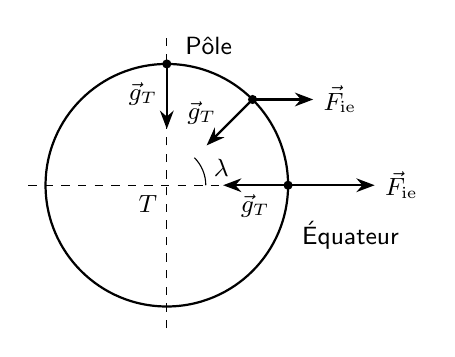
\begin{tikzpicture}[scale=1.1]
\draw[thick] (0,0) circle(1.4);\draw[dashed] (0,-1.65)--(0,1.7);\draw[dashed] (-1.6,0)--(1.6,0);\node[below left] at (0,0){$T$};
\foreach \a in {0,45,90}{\fill (\a:1.4) circle(1.5pt);\draw[->,thick] (\a:1.4)--(\a:.65);}
\node[left] at (0,1.05){$\vec g_T$};\node[below] at (1.02,0){$\vec g_T$};\node[left] at (.68,.83){$\vec g_T$};
\draw[->,thick] (1.4,0)--(2.4,0) node[right]{$\Fie$};
\draw[->,thick] (45:1.4)--++(.7,0) node[right]{$\Fie$};
\node[above right] at (.1,1.4){Pôle};\node[below right] at (1.45,-.3){Équateur};
\draw (.45,0) arc(0:45:.45);\node at (.63,.2){$\lambda$};
\end{tikzpicture}\end{center}
À l'équateur ($\lambda=0$),
\[\Omega^2HM=\Omega^2R_T\simeq3{,}2\times10^{-2}\,\mathrm{m\,s^{-2}},\qquad g_T=\frac{GM_T}{R_T^2}\simeq10\,\mathrm{m\,s^{-2}}.\]
L'effet centrifuge maximal représente environ $0{,}3\,\%$ du champ de gravitation.

\subsection{Conséquences}
\begin{center}\terre{2}\end{center}
\titr{Première conséquence}
La norme de $\vec g$ dépend de la latitude $\lambda$ : elle est minimale à l'équateur ($\lambda=0$) et maximale aux pôles ($\lambda=\pi/2$).
\[\vec g=\vec g_T+\Omega^2\HM.\]
Le théorème de Pythagore généralisé donne
\[\|\vec g\|^2=\|\vec g_T\|^2+\Omega^4R_T^2\cos^2\lambda-2g_T\Omega^2R_T\cos^2\lambda=g(\lambda)^2.\]
Les mesures donnent $g=9{,}832\,\mathrm{m\,s^{-2}}$ aux pôles et $g=9{,}780\,\mathrm{m\,s^{-2}}$ à l'équateur, soit une variation de $0{,}5\,\%$, supérieure à la valeur calculée. La Terre n'est en effet pas sphérique.

\titr{Deuxième conséquence}
$\vec g(M)$ n'est pas parallèle au rayon de la Terre. La \textbf{verticale} en un point $M$ de la surface terrestre est la direction de $\vec g(M)$ ; elle est déterminée à l'aide d'un fil à plomb.
\begin{center}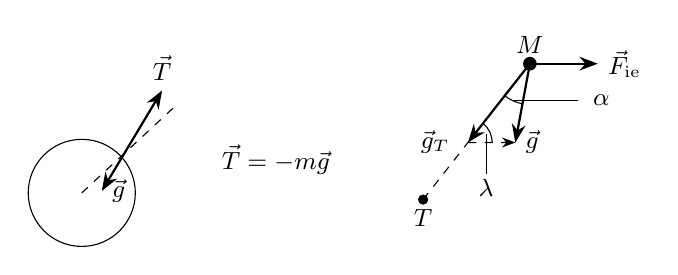
\begin{tikzpicture}[scale=.85]
\draw (0,0) circle(.8);\draw[dashed] (0,0)--(1.4,1.3);\coordinate (M) at (.6,.53);\draw[->,thick] (M)--++(.6,1) node[above]{$\vec T$};\draw[->,thick] (M)--++(-.3,-.5) node[right]{$\vec g$};\node at (2.9,.5){$\vec T=-m\vec g$};
\begin{scope}[shift={(5.1,-.1)},scale=1.45]
\coordinate (M) at (1.1,1.4);\fill (0,0) circle(1.5pt) node[below]{$T$};\draw[dashed] (0,0)--(M);\fill (M) circle(2pt) node[above]{$M$};
\coordinate (G) at ($(M)!.58!(0,0)$);\coordinate (P) at (.95,.588);
\draw[->,thick] (M)--(G) node[left,xshift=-3pt]{$\vec g_T$};
\draw[->,thick] (M)--++(.7,0) node[right]{$\Fie$};
\draw[->,thick] (M)--(P) node[right]{$\vec g$};\draw[dashed,->] (G)--(P);
\draw ($(M)+(-128.157:.42)$) arc(-128.157:-100.466:.42);
\node[right] at (1.65,1.02){$\alpha$};\draw[thin] (1.6,1.02)--(.94,1.02);
\draw ($(G)+(.25,0)$) arc(0:51.843:.25);
\node at (.65,.12){$\lambda$};\draw[thin] (.65,.26)--(.65,.68);
\end{scope}\end{tikzpicture}\end{center}
La relation des angles dans le triangle donne
\[\frac{\sin\alpha}{\om^2HM}=\frac{\sin\lambda}{g}.\]
Pour $h=0$ et $\lambda=45^\circ$, on obtient $\alpha=8'=2{,}4\times10^{-3}\,\mathrm{rad}\ll\lambda$. On néglige donc $\alpha$ devant $\lambda$.

\titr{Bilan}
$\RG$ est supposé galiléen et $\RT$ est non galiléen :
\[m\vec a_{\RT}(M)=\Fd+\underbrace{m\vec g_T(M)+m\om^2\HM}_{\vec P=m\vec g(M)}+\Fic.\]
\begin{cadre}[etoiles={\etoiles{4}}]\[m\vec a_{\RT}(M)=\Fd+m\vec g(M)+\Fic.\]\end{cadre}
Le champ $\vec g$ inclut la force d'inertie d'entraînement. La force de Coriolis dévie la trajectoire.

% Sources 15-19
\section{Influence de la force de Coriolis}
\subsection{Quelques généralités}
\[\Fic=-2m\Om\wedge\vec v_{\RT}.\]
En ordre de grandeur,
\[\frac{F_{\mathrm{ic}}}{mg}\sim\frac{2m\Omega v}{mg}.\]
Ce rapport dépasse $1\,\%$ si $v>2500\,\mathrm{km\,h^{-1}}$. La force de Coriolis intervient pour les grandes vitesses, comme celles des missiles, pour les durées longues devant $24\,\mathrm h$ ou pour les expériences précises.

\titr{Expression dans la base locale}
\begin{center}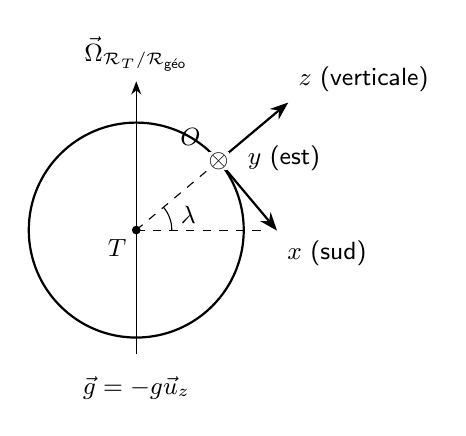
\begin{tikzpicture}[scale=1.05]
\draw[thick] (0,0) circle(1.3);\draw[->] (0,-1.5)--(0,1.8) node[above]{$\Om$};
\fill (0,0) circle(1.5pt) node[below left]{$T$};\draw[dashed] (0,0)--(1.6,0);
\coordinate (O) at (40:1.3);\draw[dashed] (0,0)--(O);
\draw (.43,0) arc(0:40:.43);\node at (.63,.18){$\lambda$};
\draw[->,thick] (O)--++(40:1.1) node[above right]{$z$ (verticale)};
\draw[->,thick] (O)--++(-50:1.1) node[below right]{$x$ (sud)};
\node[fill=white,inner sep=0pt] at (O){$\otimes$};
\node[above left,xshift=-3pt,yshift=2pt] at (O){$O$};
\node[right,xshift=7pt,yshift=1pt] at (O){$y$ (est)};
\node[below] at (0,-1.65){$\vec g=-g\uz$};
\end{tikzpicture}\end{center}
\begin{align*}
\Fic&=-2m\om\begin{pmatrix}-\cos\lambda\\0\\\sin\lambda\end{pmatrix}\wedge\begin{pmatrix}\dot x\\\dot y\\\dot z\end{pmatrix}\\
&=-2m\om\begin{pmatrix}-\dot y\sin\lambda\\\dot x\sin\lambda+\dot z\cos\lambda\\-\dot y\cos\lambda\end{pmatrix}.
\end{align*}
\begin{cadre}\[\begin{aligned}
m\ddot x&=F_{\mathrm{div},x}+2m\om\dot y\sin\lambda,\\
m\ddot y&=F_{\mathrm{div},y}-2m\om(\dot x\sin\lambda+\dot z\cos\lambda),\\
m\ddot z&=F_{\mathrm{div},z}-mg+2m\om\cos\lambda\,\dot y.
\end{aligned}\]\end{cadre}
\titr{Méthode de résolution}
On peut utiliser une méthode numérique (Python) ou une méthode par perturbation (cf. exemples de cours) :
\begin{enumerate}
\item Calculer la trajectoire en négligeant $\Fic$.
\item Calculer $\Fic$ sur la trajectoire non perturbée.
\item Réinjecter $\Fic$ dans le principe fondamental de la dynamique.
\end{enumerate}
Cette dernière méthode s'applique aux déviations très faibles.

\titr{Cas particulier des mouvements horizontaux}
Les cyclones, les anticyclones et le pendule de Foucault en sont des exemples. Pour le pendule, si $\theta\ll1$, le mouvement est quasi horizontal.
\begin{center}\pendule\end{center}
Un mouvement horizontal est perpendiculaire à la verticale : $\dot z=0$.
\begin{cadre}\[\begin{aligned}
m\ddot x&=F_{\mathrm{div},x}+2m\om\dot y\sin\lambda,\\
m\ddot y&=F_{\mathrm{div},y}-2m\om\bigl(\dot x\sin\lambda+\underbrace{\dot z\cos\lambda}_{0}\bigr).
\end{aligned}\]\end{cadre}
\[\vec F_{\mathrm{ic,hori}}=-2m\vec\Omega_{\mathrm{vert}}\wedge\vec v_{\RT,\mathrm{hori}},\qquad\vec\Omega_{\mathrm{vert}}=\Omega\sin\lambda\uz.\]
\begin{center}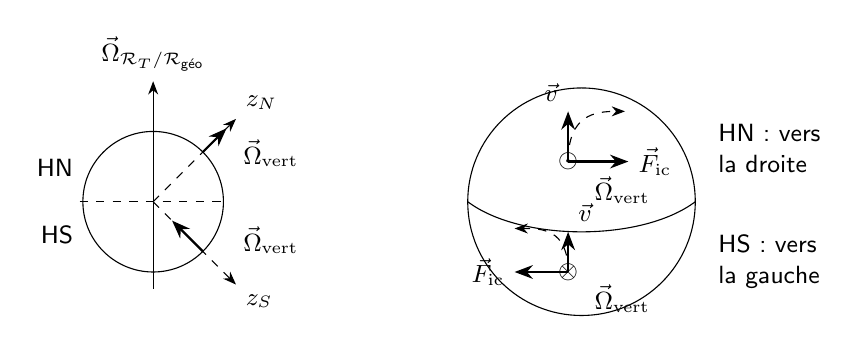
\begin{tikzpicture}[scale=.85]
\draw (0,0) circle(1.05);\draw[->] (0,-1.3)--(0,1.8) node[above]{$\Om$};
\draw[dashed] (-1.1,0)--(1.1,0);\node[left] at (-1.05,.5){HN};\node[left] at (-1.05,-.5){HS};
\draw[->,dashed] (0,0)--(45:1.75) node[above right]{$z_N$};
\draw[->,dashed] (0,0)--(-45:1.75) node[below right]{$z_S$};
\draw[->,thick] (45:1.05)--(45:1.55);\node[right] at (1.2,.72){$\vec\Omega_{\mathrm{vert}}$};
\draw[->,thick] (-45:1.05)--(-45:.4);\node[right] at (1.2,-.58){$\vec\Omega_{\mathrm{vert}}$};
\begin{scope}[shift={(6.4,0)}]
\draw (0,0) circle(1.7);\draw (-1.7,0) .. controls (-.9,-.6) and (.9,-.6) .. (1.7,0);
\coordinate (N) at (-.2,.6);\coordinate (S) at (-.2,-1.05);
\node[fill=white,inner sep=0pt] at (N){$\odot$};\node[fill=white,inner sep=0pt] at (S){$\otimes$};
\draw[->,thick] (N)--++(0,.75) node[above left]{$\vec v$};\draw[->,thick] (N)--++(.9,0) node[right]{$\Fic$};
\draw[->,dashed] (N)..controls (-.2,1.3) and (.2,1.35)..(.65,1.35);
\draw[->,thick] (S)--++(0,.6) node[above right]{$\vec v$};\draw[->,thick] (S)--++(-.8,0) node[left]{$\Fic$};
\draw[->,dashed] (S)..controls (-.2,-.4) and (-.6,-.4)..(-1,-.4);
\node[right,align=left] at (1.9,.8){HN : vers\\la droite};\node[right,align=left] at (1.9,-.9){HS : vers\\la gauche};
\node[below right] at (.05,.52){$\vec\Omega_{\mathrm{vert}}$};\node[below right] at (.05,-1.1){$\vec\Omega_{\mathrm{vert}}$};
\end{scope}
\end{tikzpicture}\end{center}

\subsection{Déviation vers l'est}
La chute libre est un mouvement quasi vertical.
\begin{center}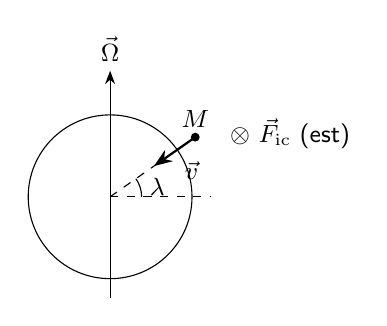
\begin{tikzpicture}[scale=.8]
\draw (0,0) circle(1.3);\draw[->] (0,-1.6)--(0,2) node[above]{$\vec\Omega$};\draw[dashed] (0,0)--(1.6,0);\coordinate (M) at (35:1.65);\draw[dashed] (0,0)--(M);\fill (M) circle(2pt) node[above]{$M$};\draw[->,thick] (M)--(35:.85) node[midway,below right]{$\vec v$};\node[right] at (1.75,1){$\otimes\ \Fic$ (est)};\draw (.5,0) arc(0:35:.5) node[midway,right]{$\lambda$};
\end{tikzpicture}\end{center}
Cf. TD 4.A.

% Sources 19-22
\subsection{Pendule de Foucault}
\begin{center}\pendule\end{center}
Pour $\theta\ll1\,\mathrm{rad}$, le mouvement est quasi horizontal. Dans l'hémisphère Nord, la déviation se fait vers la droite.
\begin{center}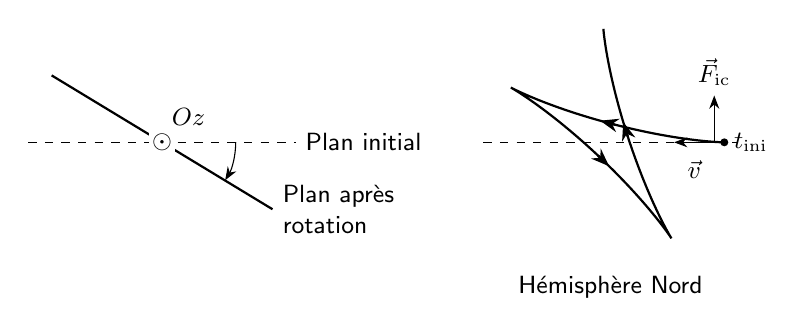
\begin{tikzpicture}[scale=.85]
\draw[dashed] (-2,0)--(2,0) node[right]{Plan initial};\draw[thick] (-1.65,1)--(1.65,-1) node[right,align=left]{Plan après\\rotation};\node[fill=white,inner sep=1pt] at (0,0){$\odot$};\node[above right] at (0,.1){$Oz$};\draw[->] (1.1,0) arc(0:-31:1.1);
\begin{scope}[shift={(6.7,0)}]
\draw[dashed] (-1.9,0)--(1.9,0);
\draw[thick]
plot[domain=0:540,samples=220,variable=\t] ({1.7*(cos(\t)*cos(.16*\t)+.16*sin(\t)*sin(.16*\t))},{1.7*(-cos(\t)*sin(.16*\t)+.16*sin(\t)*cos(.16*\t))});
\foreach \t in {90,270,450}{
\draw[->,thick] ({1.7*(cos(\t)*cos(.16*\t)+.16*sin(\t)*sin(.16*\t))},{1.7*(-cos(\t)*sin(.16*\t)+.16*sin(\t)*cos(.16*\t))})--({1.7*(cos(\t+8)*cos(.16*(\t+8))+.16*sin(\t+8)*sin(.16*(\t+8)))},{1.7*(-cos(\t+8)*sin(.16*(\t+8))+.16*sin(\t+8)*cos(.16*(\t+8)))});}
\fill (1.7,0) circle(1.7pt) node[right]{$t_{\mathrm{ini}}$};
\draw[->] (1.55,0)--(.95,0) node[midway,below=3pt]{$\vec v$};\draw[->] (1.55,0)--(1.55,.7) node[above]{$\Fic$};
\node[below] at (0,-1.85){Hémisphère Nord};
\end{scope}\end{tikzpicture}\end{center}
\[\Omega_{\mathrm{sid}}=\om,\qquad\Omega_{\mathrm{vert}}=\Omega_{\mathrm{sid}}\sin\lambda.\]
\begin{center}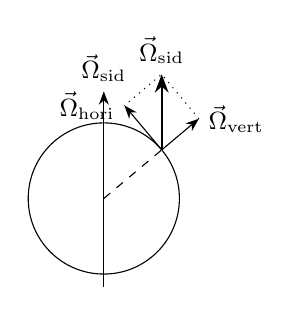
\begin{tikzpicture}[scale=.8]
\draw (0,0) circle(1.2);\draw[->] (0,-1.4)--(0,1.7) node[above]{$\vec\Omega_{\mathrm{sid}}$};\coordinate (M) at (40:1.2);\draw[dashed] (0,0)--(M);\draw[->,thick] (M)--++(0,1.2) node[above]{$\vec\Omega_{\mathrm{sid}}$};\draw[->] (M)--++(40:.77) coordinate (V) node[right]{$\vec\Omega_{\mathrm{vert}}$};\draw[->] (M)--++(130:.92) coordinate (H) node[left]{$\vec\Omega_{\mathrm{hori}}$};\draw[dotted] (V)--($(M)+(0,1.2)$)--(H);
\end{tikzpicture}\end{center}
C'est la composante verticale du vecteur rotation qui intervient dans la rotation du plan d'oscillation.
\begin{cadre}\[T_{\mathrm{rot}}=\frac{2\pi}{\Omega_{\mathrm{vert}}}=\frac{2\pi}{\Omega\sin\lambda}.\]\end{cadre}
$T_{\mathrm{rot}}$ est la période de rotation du plan d'oscillation.
\begin{center}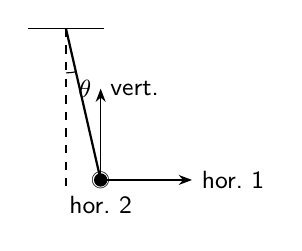
\begin{tikzpicture}[scale=.8]
\draw (-.6,0)--(.6,0);\draw[dashed] (0,0)--(0,-2.5);\draw[thick] (0,0)--(.55,-2.4);\fill (.55,-2.4) circle(3pt);\draw (0,-.7) arc(270:283:.7);\node at (.3,-.95){$\theta$};\draw[->] (.55,-2.4)--(2,-2.4) node[right]{hor. 1};\draw[->] (.55,-2.4)--(.55,-.95) node[right]{vert.};\node at (.55,-2.4){$\odot$};\node[below] at (.55,-2.5){hor. 2};
\end{tikzpicture}\end{center}
\[\Fic=-2m\vec\Omega\wedge\vec v=-2m\left[\vec\Omega_{\mathrm{vert}}+\vec\Omega_{\mathrm{hor1}}+\vec\Omega_{\mathrm{hor2}}\right]\wedge\vec v.\]
\begin{itemize}
\item $-2m\vec\Omega_{\mathrm{vert}}\wedge\vec v$ est responsable de la rotation du plan d'oscillation.
\item $-2m\vec\Omega_{\mathrm{hor1}}\wedge\vec v\simeq\vec0$, car le mouvement se fait selon la direction horizontale 1.
\item $-2m\vec\Omega_{\mathrm{hor2}}\wedge\vec v$ est vertical et modifie la tension du fil.
\end{itemize}

% Sources 22-23
\Needspace{55mm}\subsection{Anticyclones-dépressions}
On se place dans l'hémisphère Nord. Les mouvements atmosphériques sont supposés horizontaux.
\begin{center}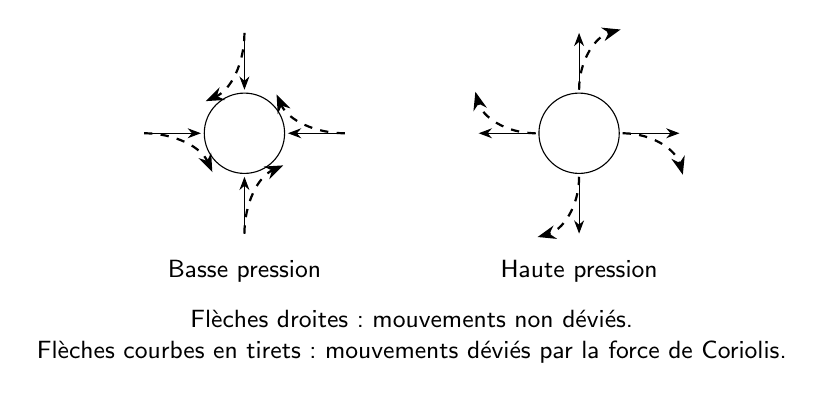
\begin{tikzpicture}[scale=.85]
\foreach \x/\name in {0/Basse pression,5/Haute pression}{\draw (\x,0) circle(.6);\node[below] at (\x,-1.75){\name};}
\foreach \a in {0,90,180,270}{
\draw[->] (\a:1.5)--(\a:.65);
\begin{scope}[rotate=\a]
\draw[->,thick,dashed] (1.5,0)..controls (1.05,0) and (.65,.2)..(.48,.58);
\end{scope}
\begin{scope}[shift={(5,0)}]\draw[->] (\a:.65)--(\a:1.5);\begin{scope}[rotate=\a]
\draw[->,thick,dashed] (.65,0)..controls (1.1,0) and (1.45,-.25)..(1.55,-.62);
\end{scope}\end{scope}}
\node[below,align=center] at (2.5,-2.5){Flèches droites : mouvements non déviés.\\Flèches courbes en tirets : mouvements déviés par la force de Coriolis.};
\end{tikzpicture}\end{center}
\begin{center}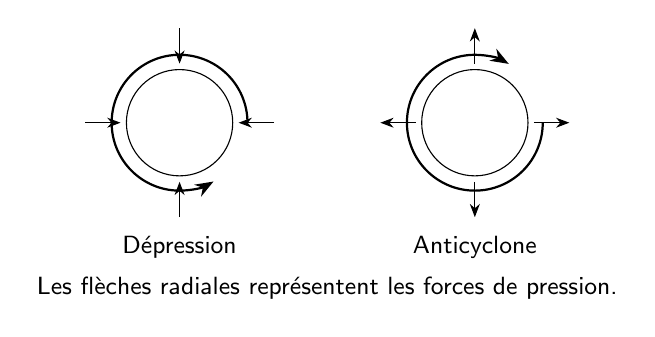
\begin{tikzpicture}[scale=.75]
\foreach \x in {0,5}{\draw (\x,0) circle(.9);}
\draw[->,thick] (1.15,0) arc(0:300:1.15);\draw[->,thick] (6.15,0) arc(0:-300:1.15);
\foreach \a in {0,90,180,270}{\draw[->] (\a:1.6)--(\a:1);\begin{scope}[shift={(5,0)}]\draw[->] (\a:1)--(\a:1.6);\end{scope}}
\node[below] at (0,-1.75){Dépression};\node[below] at (5,-1.75){Anticyclone};\node[below] at (2.5,-2.45){Les flèches radiales représentent les forces de pression.};
\end{tikzpicture}\end{center}
À l'équilibre géostrophique, $\Fic=-\vec F_{\mathrm{pression}}$. Les dépressions tournent dans le sens trigonométrique et les anticyclones dans le sens horaire. Les sens sont inversés dans l'hémisphère Sud.

Les cellules de Hadley correspondent à des courants de convection de l'air.
\begin{center}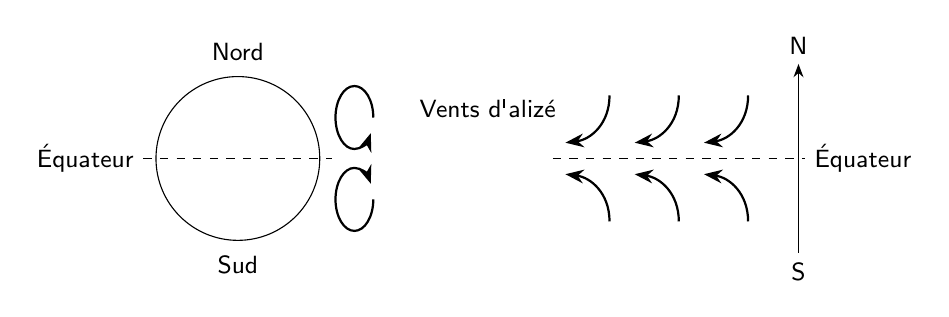
\begin{tikzpicture}[scale=.8]
\draw (0,0) circle(1.3);\draw[dashed] (-1.5,0)--(1.5,0);\node[left] at (-1.5,0){Équateur};\node[above] at (0,1.4){Nord};\node[below] at (0,-1.4){Sud};
\draw[->,thick] (2.15,.65) arc(0:330:.3 and .5);
\draw[->,thick] (2.15,-.65) arc(0:-330:.3 and .5);
\begin{scope}[shift={(7,0)}]\draw[->] (1.9,-1.5)--(1.9,1.5) node[above]{N};\node[below] at (1.9,-1.5){S};\draw[dashed] (-2,0)--(2,0) node[right]{Équateur};\foreach \x in {-1.1,0,1.1}{\draw[->,thick] (\x,1)..controls (\x,.55) and ({\x-.3},.3)..({\x-.7},.25);\draw[->,thick] (\x,-1)..controls (\x,-.55) and ({\x-.3},-.3)..({\x-.7},-.25);}\node[left] at (-1.8,.8){Vents d\textquotesingle alizé};\end{scope}
\end{tikzpicture}\end{center}
% Sources 23-28
\section{Effets de marées}
\subsection{Le terme des marées}
\begin{center}\orbite{0}\end{center}
On suppose $\RH$ galiléen. Le référentiel d'étude est $\RG$, avec $\vec\Omega_{\RG/\RH}=\vec0$.
Le système est une particule de fluide, de masse $m$, située en $M$, dans l'océan à la surface terrestre.

Dans la théorie statique des marées, on suppose que cette particule d'eau est en équilibre dans $\RT$. Elle décrit donc dans $\RG$ un mouvement circulaire uniforme autour de $\Delta$, l'axe des pôles.

\Needspace{30mm}
Le théorème de la quantité de mouvement, ou principe fondamental de la dynamique, appliqué à cette particule dans $\RG$, donne
\[m\vec a_{\RG}(M)=\Fd+\underbrace{m\vec g_T(M)}_{\text{gravitation de la Terre}}+\underbrace{m\sum_a\vec g_a(M)}_{\text{gravitation des autres astres}}+\Fie+\Fic.\]
Dans le cas où $\RG$ est en translation par rapport à $\RH$,
\[m\vec a_{\RG}(M)=-m\om^2\HM,\qquad\Fic=\vec0,\]
\[\Fie=-m\vec a_e(M)=-m\vec a_{\RH}(T).\]
Ainsi,
\[-m\om^2\HM=\Fd+m\vec g_T(M)+m\sum_a\vec g_a(M)-\underbrace{m\vec a_{\RH}(T)}_{\text{à déterminer}}.\]
Le théorème de la quantité de mouvement appliqué à la Terre dans $\RH$ donne
\[M_T\vec a_{\RH}(T)=\sum_aM_T\vec g_a(T),\qquad\vec a_{\RH}(T)=\sum_a\vec g_a(T).\]
On suppose ici $\vec g_a$ uniforme sur la Terre : $R_T\ll D_a$, où $D_a$ est la distance entre la Terre et l'astre.

En combinant ces relations,
\[\vec0=\Fd+\underbrace{m\vec g_T(M)+m\om^2\HM}_{m\vec g(M)}+\sum_a m\vec g_a(M)-m\sum_a\vec g_a(T).\]
\begin{cadre}\[\vec0=\Fd+\underbrace{m\vec g(M)}_{\text{pesanteur terrestre}}+m\underbrace{\left[\sum_a\bigl(\vec g_a(M)-\vec g_a(T)\bigr)\right]}_{\text{terme des marées}}.\]\end{cadre}
Le terme des marées est dû aux mouvements de la Terre dans l'espace.

\titr{Ordres de grandeur}
\begin{center}\maree{0}\end{center}
On suppose que l'astre $A$ possède une symétrie sphérique. Le champ gravitationnel créé est le même que celui d'une masse ponctuelle $M_A$ située en $A$.

Le champ $\vec g_a(M)-\vec g_a(T)$ est le \textbf{champ différentiel des marées}.
\begin{center}\maree{1}\end{center}
Pour estimer son ordre de grandeur, étudions $\vec g_a$ en $P$ et en $Q$. Puisque $R_T\ll D_A$, on effectue un développement limité en $R_T/D_A$.

En $Q$ :
\begin{align*}
\|\vec g_a(Q)-\vec g_a(T)\|
&=\left|\frac{GM_A}{(D_A-R_T)^2}-\frac{GM_A}{D_A^2}\right|\\
&=\frac{GM_A}{D_A^2}\left|\frac1{\left(1-\dfrac{R_T}{D_A}\right)^2}-1\right|\\
&\simeq\frac{GM_A}{D_A^2}\left(\frac{2R_T}{D_A}\right).
\end{align*}
En $P$ :
\begin{align*}
\|\vec g_a(P)-\vec g_a(T)\|
&=\left|\frac{GM_A}{(D_A+R_T)^2}-\frac{GM_A}{D_A^2}\right|\\
&=\frac{GM_A}{D_A^2}\left|\frac1{\left(1+\dfrac{R_T}{D_A}\right)^2}-1\right|\\
&\simeq\frac{GM_A}{D_A^2}\left(\frac{2R_T}{D_A}\right).
\end{align*}
Donc,
\begin{cadre}[etoiles={\etoiles{3}}]\[g_{d,\max}=\frac{2GM_AR_T}{D_A^3}.\]\end{cadre}
Les trois étoiles portent sur le calcul. La Lune est l'astre le plus proche : l'effet prépondérant vient de la Lune, avec un ordre de grandeur de $10^{-6}\,\mathrm{m\,s^{-2}}$.
\[\vec0=\Fd+m\vec g_T(M)+m\om^2\HM+m\sum_a\left[\vec g_a(M)-\vec g_a(T)\right].\]
Les ordres de grandeur des champs correspondants sont :
\begin{center}\begin{tabular}{ll}
Gravitation terrestre & $10\,\mathrm{m\,s^{-2}}$\\[3pt]
Terme centrifuge & $3\times10^{-2}\,\mathrm{m\,s^{-2}}$\\[3pt]
Terme des marées lunaires & $\sim10^{-6}\,\mathrm{m\,s^{-2}}$\\[3pt]
Terme des marées solaires & $\sim5\times10^{-7}\,\mathrm{m\,s^{-2}}$
\end{tabular}\end{center}

% Sources 28-32
\subsection{Théorie statique des marées}
\begin{center}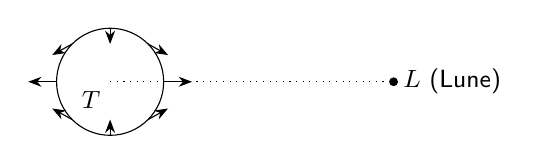
\begin{tikzpicture}[scale=.8]
\draw (0,0) circle(.85);\node[below left] at (0,0){$T$};\draw[dotted] (0,0)--(4.5,0);\fill (4.5,0) circle(2pt) node[right]{$L$ (Lune)};
\foreach \a in {0,45,90,135,180,225,270,315}{\draw[->] (\a:.85)--++({.45*cos(\a)},{-.25*sin(\a)});}
\end{tikzpicture}\end{center}
\begin{center}\maree{2}\end{center}
Deux bourrelets océaniques se forment, de hauteur de l'ordre de quelques mètres. Ils sont très petits devant $R_T$, mais visibles à notre échelle.
\begin{center}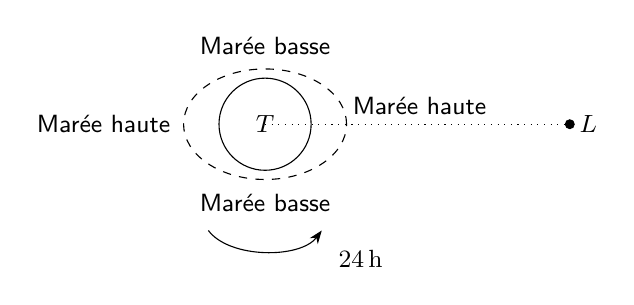
\begin{tikzpicture}[scale=.9]
\draw (0,0) circle(.65);\draw[dashed] (0,0) ellipse(1.15 and .78);\draw[dotted] (0,0)--(4.3,0);\fill (4.3,0) circle(2pt) node[right]{$L$};\node at (0,0){$T$};
\node[above] at (0,.85){Marée basse};\node[below] at (0,-0.85){Marée basse};\node[left] at (-1.2,0){Marée haute};\node[above right] at (1.1,0){Marée haute};
\draw[->] (-.8,-1.5) .. controls (-.5,-1.9) and (.5,-1.9) .. (.8,-1.5);\node[right] at (.9,-1.9){$24\,\mathrm h$};
\end{tikzpicture}\end{center}
La période de rotation de la Lune autour de la Terre est d'environ $27$ jours. La Lune est donc supposée fixe sur les $24\,\mathrm h$ d'un jour.

\begin{center}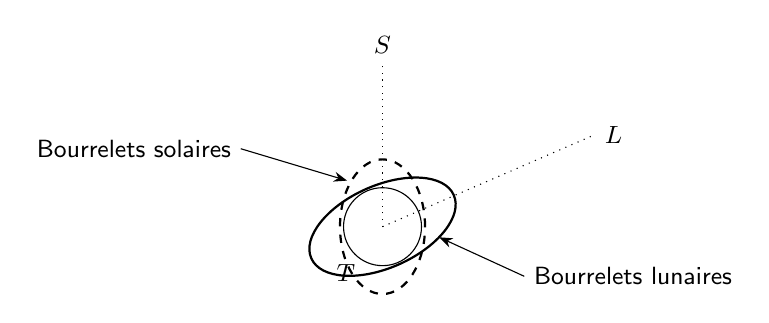
\begin{tikzpicture}[scale=.9]
\draw (0,0) circle(.55);\node[below left] at (-.25,-.4){$T$};\draw[dotted] (0,0)--(0,2.3) node[above]{$S$};\draw[dotted] (0,0)--(3,1.3) node[right]{$L$};\draw[thick,rotate=24] (0,0) ellipse(1.1 and .58);\draw[thick,dashed] (0,0) ellipse(.6 and .95);
\draw[->] (2,-.7) node[right]{Bourrelets lunaires}--(.8,-.15);\draw[->] (-2,1.1) node[left]{Bourrelets solaires}--(-.5,.65);
\end{tikzpicture}\end{center}
À la pleine lune et à la nouvelle lune, $L$, $T$ et $S$ sont alignés : ce sont les \textbf{marées de vives-eaux}.
Aux quartiers de lune, les effets de la Lune et du Soleil se compensent : ce sont les \textbf{marées de mortes-eaux}.

\titr{Pour une étude plus complète}
\begin{itemize}
\item La théorie dynamique prend en compte une force excitatrice périodique, en régime forcé.
\item Il faut étudier les ondes de propagation des marées et leur temps de réponse.
\item La présence des continents décale les marées dans le temps. La théorie statique prévoit $30$ minutes de décalage entre Brest et Deauville. En pratique, le décalage est de $8\,\mathrm h$, comme le prédit la théorie dynamique.
\item Les continents entraînent des effets de résonance : environ $10\,\mathrm m$ de marée au Mont-Saint-Michel et environ $20\,\mathrm m$ au Canada.
\item Les marées solides entraînent une variation de $1\,\mathrm{mm}$ du périmètre du grand accélérateur de Genève, long de $27\,\mathrm{km}$. Une comète subit aussi les effets de marée lorsqu'elle passe près d'une planète : elle se brise si elle passe trop près et que les champs de marée sont trop importants. Ce phénomène est à l'origine des anneaux des planètes.
\item Les marées Lune--Terre ralentissent la rotation terrestre. Il y a $400$ millions d'années, un jour durait $22\,\mathrm h$. La durée du jour augmente de $1{,}6\times10^{-3}\,\mathrm s$ par siècle.
La Lune est ralentie par la Terre et présente toujours la même face à la Terre.
\end{itemize}
\end{document}